
\chapter{Additional Results}
\label{c.discussion}

The previous chapters demonstrated a widespread potential for
coordination avoidance in existing applications and semantics. This in
turn led to several algorithmic advances that enabled high-performance
implementations of these semantics.  The results we have discussed
thus far were enabled by the exploration of several related questions,
which we describe below. While we omit a comprehensive treatment of
these additional results, we believe that the discussion below
addresses several important issues of interest related to
coordination-avoiding systems.


\section{Quantifying Eventual Consistency} 

Many coordination-free data stores as deployed in production today do
not provide any safety guarantees. Instead, these data stores promise
\textit{eventual consistency}, which guarantees that eventually---in
the absence of new writes, at some future time unknown in
advance---all replicas of each data item will {\em converge} to the
same value~\cite{vogels-defs}. Eventual consistency is a {\em
  liveness} property, which ensures that something good will
eventually happen (replicas agree)~\cite{liveness}. It does not
provide {\em safety} guarantees: it is impossible for a system to
violate eventual consistency at any discrete moment because the system
may converge in the future~\cite{queue}. Despite eventual
consistency's lack of safety, data store operators frequently choose
this
option~\cite{cassandra-docs,cassandradefault,feinbergpc,reddit,outbrain,maxperfblog}---an often controversial
decision~\cite{hamilton-cap,cops,walter,urbanmyths}.  Given their
performance benefits, which are especially important as latencies
grow~\cite{pacelc,feinbergpc,hamilton-cap,helland},
eventually consistent store configurations are often considered
acceptable.  The proliferation of eventually consistent deployments
suggests that applications can often tolerate occasional staleness and
that query results tend to be ``fresh enough'' in many cases.

While common practice suggests that eventual consistency is often a
viable solution for data store operators, this observation was largely
anecdotal. In this work, we quantified the degree to which eventual
consistency is both eventual and consistent and explained why. Under
worst-case conditions, eventual consistency results in an unbounded
degree of data staleness, but, as we demonstrated, the average case is
often different.  Eventually consistent data stores cannot promise
safety but, for varying degrees of certainty, can offer staleness
bounds with respect to time (``how eventual'') and versions (``how
consistent'').

There was little prior work describing how to make these consistency
and staleness predictions under practical conditions.  The prior
state of the art required that users make rough guesses or perform
online profiling to determine the consistency provided by their data
stores~\cite{bermbach-eventual,podc-hpl,wada-data}. Users
had little to no guidance on how to choose an appropriate replication
configuration or how to predict the behavior of eventual consistency
in production environments.

To predict consistency, we need to know when and why eventually
consistent systems return stale data and how to quantify the staleness
of the data they return.  In response, we developed algorithms and
models for predicting the staleness, called Probabilistically Bounded
Staleness (PBS)~\cite{pbs,pbs-vldbj2013,pbs-demo-sigmod2013}. There are two common metrics for measuring staleness
in the literature: wall clock
time~\cite{podc-hpl,timed-consistency,yu-conit,vahdat-bounded}
and versions~\cite{podc-hpl,aqua,frac}.  PBS describes both measures,
providing the probability of reading a write $\Delta$ seconds after it
returns ($(\Delta, p)$-semantics, or ``how eventual is eventual
consistency?''), of reading one of the last $K$ versions of a data
item ($(K, p)$-semantics, or ``how consistent is eventual
consistency?''), and of experiencing a combination of the two ($(K,
\Delta, p)$-semantics). PBS does not propose new mechanisms to enforce
deterministic staleness
bounds~\cite{aqua,trapp,yu-conit,vahdat-bounded,frac}; instead,
our goal is to provide a lens for analyzing, improving, and predicting
the behavior of \textit{existing}, widely deployed systems.

We used PBS to examine the latency-consistency trade-off in the
context of quorum-replicated data stores such as Dynamo~\cite{dynamo}
and its open source descendants Apache
Cassandra~\cite{cassandra-sigmod}, Basho Riak~\cite{riak}, and Project
Voldemort~\cite{voldemortpub}. Quorum systems ensure regular register
semantics across reads and writes to replicas by ensuring that read
and write replica sets overlap. However, employing \textit{partial}
(or non-strict) quorums can lower latency by requiring fewer replicas
to respond.  With partial quorums, sets of replicas written to and
read from need not overlap: given $N$ replicas and read and write
quorum sizes $R$ and $W,$ partial quorums imply $R$$+$$W$$\leq$$N$.

\begin{figure}
\centering
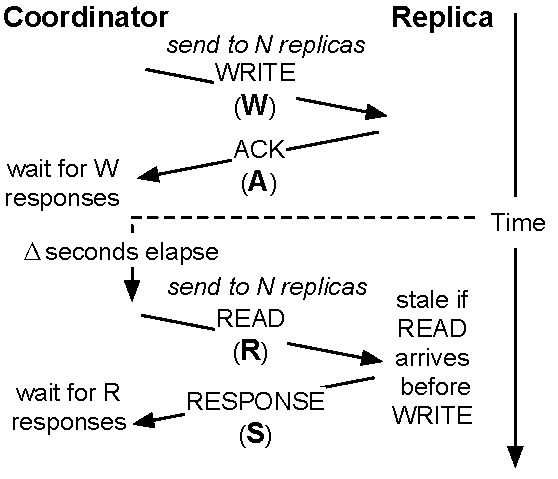
\includegraphics[width=.5\columnwidth]{figs/dynamostale.pdf}\vspace{.5em}
\caption{The \textit{WARS} model for Dynamo-style quorum systems
  describes the message latencies between a coordinator and a single
  replica for a write followed by a read $t$ seconds after commit.  In
  an $N$ replica system, this messaging occurs $N$ times. We use this
  model to evaluate $(\Delta, p)$-regular semantics in PBS based on
  empirical distributions for each of \textit{W}, \textit{A},
  \textit{R}, and \textit{S}.}
\label{fig:dynamo-diagram}
\end{figure}


We built upon prior work on \textit{probabilistic
  quorums}~\cite{prob-quorum,quorum-overview} to account for
multi-version staleness and messaging protocols as used in today's
systems. We derived closed-form solutions for PBS $(K, p)$-regular
semantics and use Monte Carlo methods to explore the trade-off between
latency and $(\Delta, p)$-regular semantics (Figure~\ref{fig:pbs-wars}). Using production latency
distributions, we presented a detailed study of Dynamo-style PBS
$(\Delta, p)$-regular semantics. We demonstrated how long-tailed
one-way write latency distributions affect the time required for a
high probability of consistent reads.  For example, in one production
environment, switching from spinning disks to solid-state drives
dramatically improved consistency (e.g., $1.85$ms versus $45.5$ms wait
time for a $99.9$\% probability of consistent reads) due to decreased
write latency mean and variance.  We also developed quantitative
observations of the latency-consistency trade-offs offered by partial
quorums.  For example, in another production environment, we observe
an $81.1\%$ combined read and write latency improvement at the
$99.9$th percentile ($230$ to $43.3$ms) for a $202$ms window of
inconsistency ($99.9\%$ probability consistent reads). This analysis
demonstrates the performance benefits that lead operators to choose
eventual consistency.

Thus, this work offers the following contributions:
\begin{itemize}

\item We develop the theory of Probabilistically Bounded Staleness
  (PBS) for partial quorums. PBS can describe the probability of
  staleness across versions ($(K, p)$-semantics) and time ($(\Delta,
  p)$-semantics) as well as the probability of session-based consistency.

\item We provide a closed-form analysis of $(K, p)$-regular semantics
  for quorum systems and demonstrate how the probability of receiving
  data $k$ versions old is exponentially reduced by $k$.  As a
  corollary, $(K, p)$-regular semantics tolerance also exponentially
  lowers quorum system \textit{load}.

\item We introduce the \textit{WARS} model for $(\Delta, p)$-regular
  semantics in Dynamo-style partial quorum systems and show how
  message reordering leads to staleness.  We evaluated the $(\Delta,
  p)$-regular semantics of Dynamo-style systems using a combination of
  synthetic and production latency models.

\item We present theoretical and empirical analysis for the
  likelihood of two kinds of multi-key operations: transactional
  atomicity and causal consistency. We evaluate the probability of
  causal consistency using real-world workloads and also describe our
  experiences in integrating the PBS predictor in production data
  stores.
\end{itemize}

\section{Upgrading Safety using the Bolt-On Architecture}

While PBS showed how eventually consistent stores often deliver
consistent results, these stores still sometimes surface
``inconsistent'' behavior due to lack of safety guarantees. If users
want stronger guarantees, stores may provide stronger models that, in
addition to convergence, provide safety. However, exact guarantees
differ across stores and sometimes between releases of the same
stores. Can we prevent unsafe behavior without negating existing
stores' benefits, and can we do so without directly modifying existing
systems?

%% But many provide some sort of atomic consistency, which becomes
%% unavailable when partitions occur.

%% ALIG: The below paragraph is a bit odd, it makes the argument that
%% once you picked a store, you locked yourself to a consistency
%% model. I don't think we should lead with this argument. 

%% Modern data stores typically provide a small, fixed subset of the many
%% distributed consistency models, and the choice of store dictates the
%% consistency model for the application
%% programmer~\cite{windowsazurestorage, bigtable, dynamo, gfs,
%%   cassandra}. As a consequence, users often cannot easily migrate away
%% from weaker models in the event of misbehavior or relax their chosen
%% consistency in favor of better performance without changing
%% stores. Further, a growing array of consistency models and
%% implementations~\cite{pbs, practi, pnuts, cops,depot, walter,
%%   sessionguarantees} litters the design space, complicating the
%% trade-off.

We developed a general approach that separates architectural concerns
of liveness, replication, and durability from the semantics of
safety-related data consistency~\cite{bolton}. Our approach treats
consistency-related safety as a \textit{bolt-on} property provided by
a shim layer on top of a general-purpose data store. This allows a
clean, layered separation of safety and liveness concerns: the
underlying store is responsible for liveness, replication, durability,
and convergence, which require substantial engineering effort to make
practically usable. Safety properties, which are algorithmic in nature
and often hard to implement correctly, are kept separate and located
in a separate layer atop the general-purpose store. This enables a
shim to provide the exact same consistency model regardless of the
implementation or semantics of the underlying store, even if provided
as an online service (e.g., DynamoDB). This architecture can also lead
to standardized implementations that bring clarity and portability to
distributed consistency, a design space occupied by an array of custom
implementations that often differ only slightly in the consistency
guarantees they provide.

%% The bolt-on approach is inspired by Florescu and Kossman's ``new
%% [layered] architecture'' for internet service
%% databases~\cite{kraska-s3, kossman-arch}, and, in this work, we
%% formalize and further develop their proposal in the context of weakly
%% consistent ``NoSQL'' stores.

%% This allows component reuse, enables flexibility in using different
%% consistency models, and simplifies system design---we perform safety
%% checking at the system endpoints rather than require it at all
%% layers. Reliability, availability, convergence, and propagation are
%% all handled by a simple back-end, while a narrow shim layer between
%% clients and the data store provides consistency via safety guarantees.


\begin{figure}[t!]
\centering
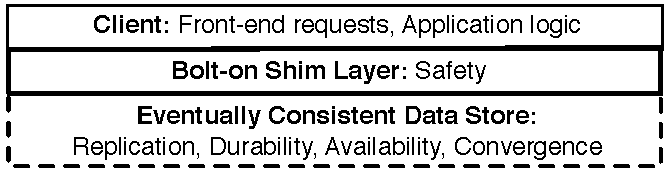
\includegraphics[width=.6\columnwidth]{figs/sep-concerns.pdf}\vspace{1em}
\caption{Separation of concerns in the bolt-on architecture. In this
  work, a narrow shim layer upgrades an underlying
  eventually consistent data store to provide causal consistency.}
\label{fig:sepconcerns}
\end{figure}

As a first step in the direction of the general approach outlined
above, we developed a bolt-on architecture to provide causal
consistency on top of eventually consistent stores (Figure
~\ref{fig:sepconcerns}). As we have discussed, causal consistency
guarantees that reads will obey causality relationships between
writes: if one event ``influences'' a subsequent operation, a client
cannot observe the second without the first~\cite{causalmemory,
  lamportclocks}.  Our choice of causal consistency is motivated by
several recent developments. Multiple ``NoSQL'' stores have added
stronger consistency, implying that there is a demand for consistency
guarantees that are stronger than eventual~\cite{simpledb}. However,
service availability is crucial for many applications, as many
companies observe negative business impact in the face of
unavailability or increased latency~\cite{amazon-latency}. We upgrade
one of the weakest coordination-free models---eventual---to one of the
strongest.  Moreover, causal consistency allows purely local reads,
enabling better performance than stronger models that often require
inter-replica communication on every operation. As a final, more
pragmatic motivation, while there has recently been considerable
academic interest in causal consistency~\cite{explicit-socc, cops,
  cac}, no production-ready data stores provide it, so bolt-on causal
consistency fills a gap in current technology.

There are two main challenges in providing causal consistency in a
bolt-on architecture: handling overwritten histories and maintaining
availability. First, when there are multiple writes to a given data
item, the eventually consistent store often chooses a single, winning
write. Attempting to directly use existing algorithms for causal
consistency~\cite{causalmemory, practi, lazyreplication, cops, cbcast} by using the underlying store as a communication medium will
fail because the bolt-on layer is not guaranteed to see all writes. We
refer to this as the problem of {\em overwritten histories}, or lost
metadata due to data store overwrites.
%
Second, we need to ensure that the shim maintains availability (one of
the key benefits of causal consistency) in the presence of
partitions. The shim should never block waiting for a causal
dependency that is either delayed or may never arrive (due to
overwritten histories). If we employ an existing algorithm that
assumes reliable write delivery, then the shim will either become
unavailable or lose convergence properties in the presence of
overwrites.

The main innovation in our bolt-on shim is an algorithm that buffers
writes and ensures that each write satisfies the criteria for a {\em
  causal cut} across the writes it has observed. By developing a
declarative specification for causal cuts, we determine what writes to
either synchronously or asynchronously fetch from the underlying data
store as well as what metadata to store with each write. Only when a
causal cut is satisfied are writes made visible to shim clients. This
guarantees that the shim is always causally consistent, convergent,
and coordination-free.

In this work, we made the following contributions:
\begin{itemize}
\item We describe a system architecture for achieving convergent causal
  consistency by applying a narrow bolt-on shim layer to an eventually
  consistent data store.

\item We present a solution to the problem of overwritten histories,
  which arises from most eventually consistent stores' register
  semantics. Solving this problem key to achieving convergent bolt-on
  causal consistency and requires a generalized, declarative
  specification for causal consistency.

\item We evaluate our shim implementation on top of
  Cassandra~\cite{cassandra-sigmod}, a production-ready eventually consistent
  data store, using real-world \textit{explicit causal consistency}
  traces. For many traces, we achieve peak throughput within a factor
  of two and often within 25\% of eventually consistent operation,
  and, for one variant of bolt-on causal consistency, outperform
  default eventually consistent operation.

\end{itemize}

\section{Specifying Application Criteria} 
\label{sec:explicitcausality}

During our development of the bolt-on shim, we examined the use of
application-provided causal dependencies in lieu of classic
process-level causal dependencies. Specifically, we identified a
critical trade-off between write throughput and visibility latency, or
the amount of time that each write is hidden from readers due to
missing dependencies that have yet to propagate. This trade-off is
influenced by two factors: the number of datacenters (or processes)
and the rate at which each datacenter can check dependencies and apply
new writes. First, scaling the number of datacenters does not improve
throughput: causal dependencies are not cleanly partitionable and must
be sent to all datacenters, limiting sustainable throughput to that of
the slowest datacenter (effectively zero in the event of network
partitions)---or, alternatively, requiring unbounded visibility
latency. Scaling total throughput while adding more datacenters
requires quadratic increases in total server capacity. Second, each
datacenter must buffer each write until it has observed all of the
write's dependencies. This phenomenon is well documented~\cite{catocs}
but is amplified by the enormous causal dependency graphs of modern
services. Combined, these effects result in either severe peak write
throughput limitations or unacceptably high visibility latency.

While these dangers are potentially prohibitive to the success of
causal consistency, we can decrease their severity by considering
modern application contexts. In the three decades since Lamport's
seminal work defining the causal \texttt{happens-before}
relation~\cite{lamportclocks}, both practitioners and theoreticians
have almost exclusively considered the problem of \textit{potential
  causality}: each new write causally depends on all writes (versions)
that could have influenced it. This is a useful model for closed
systems and debugging but is too general for modern real-world
applications. Steve's latest Facebook comment was potentially
influenced by the hundreds of status updates he had recently read, but
its primary dependency is Mary's wall post---to which his comment is
attached---asking if he was planning to attend her party.

Modern, human-facing services already naturally express semantic
dependencies in their APIs and the data they produce; in many cases we
can use these application-level relationships to explicitly define
relevant dependencies instead of having the system assume all
potential causality patterns~\cite{explicit-socc}. This
application-defined \textit{explicit
  causality}~\cite{catocs,lazyreplication,fekete99} is a small subset
of traditional potential causality and dramatically reduces the depth
and degree of the causality graph, ameliorating scalability
concerns. To quantitatively illustrate these effects, we drew on a
substantial body of literature studying behavior patterns in modern
Internet services. Studies show that explicit causality graphs for
these services are often in the tens of events and seldom in the
hundreds or thousands of events. As an example, Twitter conversation
lengths average approximately $11$ Tweets~\cite{ritter-twitter-study,
  ye-twitter-study}. In contrast, if we capture the potential
causality for a year's worth of Tweets, the resulting causality graph
is around nine orders of magnitude larger.

Prior work by Cheriton and Skeen denounced the semantics and
scalability of causally ordered communication systems (i.e.,
CATOCS)~\cite{birman-response, catocs}; in light of recent interest,
we revisited their concerns in the context of causally consistent
\textit{data stores}. We embrace Cheriton and Skeen's position that a
communication system is ill-suited to express or capture
\textit{data-level} dependencies and believe these dependencies are
best captured at or above the storage level, where many of today's
systems share data.  While our causally consistent data storage
provides a more natural model, it presents new pitfalls and requires a
different approach.

Explicit causality is not a perfect solution, yet it helps mitigate
many of the difficulties operators will face in providing causal
consistency. Explicit causality decreases the number of dependencies
per write, which increases throughput, lowers metadata overhead
(particularly in the presence of partitions), and improves
concurrency. Many dependencies are already captured by applications
and present in their data models; adopting explicit causality is often
transparent or is a simple extension to many applications. Explicit
causality does not solve the fundamental problems of all-to-all
replication or guaranteed graceful partition tolerance but instead
reduces constant factor overheads by several orders of
magnitude. Given these scalability improvements and ease of use in
modern applications, we believe explicit causality will be a key
component in achieving causal consistency at scale under real-world
conditions.

\section{Coordination-Free Analytics}
\label{sec:cf-analytics}

Until now, we have largely concerned ourselves with coordination-avoiding
data serving and transaction processing. However, as the result of
substantial collaborations with colleagues in machine learning, we
have begun to apply coordination-avoiding systems design to
optimization routines.

\minihead{Asynchronous Convex Optimization via Plasma} The recent rise
of large-scale distributed dataflow frameworks has enabled widespread
adoption of increasingly sophisticated analytics tasks at
scale~\cite{carey-bigdata,spark,stratosphere,mapreduce,dryad}. The
last decade has seen considerable research and industrial effort put
towards understanding how to integrate complex analytics and learning
tasks into programmer workflows~\cite{chris-feature,mlbase}, existing
system architectures~\cite{bismarck,madlib}, and new cluster compute
frameworks~\cite{mli,vowpal}.

% complex statistical analytics: shift towards asynchrony
% intuition: fine-grained sharing is okay
% intuition: robustness in statistical processes okay

Simultaneously, in the machine learning community, the statistical
nature of many of these analytics tasks has led to increasing interest
in exploiting \textit{asynchrony} during computation. That is, a range
of recent theoretical results has demonstrated that removing
synchronization within an emerging class of problems can yield surprising
improvements in performance. These problems can be
solved via highly concurrent update mechanisms that expose, in effect,
read-write race
conditions~\cite{dual-averaging,hogwild-coorddescent,shalev-accelerated}. As
an example, Recht et al. have demonstrated that stochastic gradient
descent---typically implemented via serializable locking (and only
proven to converge under serial execution)---can be made robust
against asynchronous processing over shared, mutable model state: in
effect, when conflicts are rare (enough), (some) staleness and data
races will not affect statistical
correctness~\cite{hogwild}. Empirically, on single-node systems, these
asynchronous algorithms have yielded order-of-magnitude improvements
in performance and are the subject of active research, even within the
database community~\cite{bismarck,dimmwitted,sgd-matrix}.

% has lead to a new class of systems
% tension: new systems but widely-deployed dataflow
% tension: distributed vs. non-distributed
% tension: unclear if it will even work

Unfortunately, these two trends stand in opposition. Architecturally,
commodity distributed dataflow systems such as Hadoop and Spark are
optimized for coarse-grained (often bulk synchronous
parallel~\cite{valiant-bsp}) data transformations and are not designed
to natively provide the fine-grained communication required for
efficient asynchronous analytics tasks. Consequently, evaluation of
these new asynchronous algorithms have been largely confined to
single-node, multi-processor (and NUMA)
context~\cite{dimmwitted,hogwild}: it is relatively unknown how the
increased latency of a distributed environment impacts their
performance and correctness guarantees. The technological trajectory
outlined by recent research suggests a divide between
widely-deployed dataflow-based cluster compute frameworks and
specialized asynchronous optimization mechanisms, which largely rely
on a shared memory abstraction~\cite{parameter-server,stale-parameter,yahoo-lda}.


% two related questions: what are the architectural implications of fine-grained
% information sharing in a dataflow engine and what, if any, are the benefits?

We studied this disconnect by addressing two key
questions~\cite{admm}.  First, can increasingly ubiquitous dataflow systems be
easily adapted to support asynchronous analytics tasks?  Second, in a
distributed dataflow environment, what are the benefits (and costs) of
these asynchronous algorithms compared with existing synchronous
implementations?  We present the design and evaluation of a simple
dataflow operator that $i.)$ enables implementation of asynchronous
complex statistical analytics (primarily, \textit{convex programming}
tasks, including Support Vector Machines and Logistic
Regression~\cite{boyd-book}) yet $ii.)$ is implementable using a
commodity dataflow engine (Apache Spark). We use this operator to
study the implications of bringing distributed asynchrony to two
classic convex programming procedures: stochastic gradient descent
(SGD)~\cite{boyd-book} and alternating direction method of multipliers
(ADMM)~\cite{boyd-admm}. This juxtaposition of traditional BSP systems
and algorithms with their incipient asynchronous counterparts yields
an opportunity to study the differences between these paradigms.

% in this paper: fine-grained dataflow for an existing engine
% intra-operator parallelilsm; bushy is not enough: often a
% single-stage dataflow
% extend iterator model to include exchange operator (interchange)
% idea one: exchange operator

\begin{figure}
\includegraphics[width=.7\linewidth]{figs/BAP-pattern.pdf}\vspace{.5em}
\caption{ASIP Iterator Architecture. A set of shared-nothing dataflow operators
  communicate asynchronously via a shared ASIP iterator, allowing
  efficient and concise implementation of complex analytics tasks
  without compromising the core dataflow abstraction.}
\label{fig:bap-architecture}
\end{figure}
To address the first, architectural question, we codify and exploit a
common pattern in asynchronous analytics tasks. We observe that, on a
single machine, these tasks can be cast as single-stage parallel
dataflow, with shared memory acting as a communication channel between
operators. Therefore, to allow asynchronous data sharing during
distributed operation, we introduce the Asynchronous Sideways
Information Passing (ASIP) pattern, in which a set of shared-nothing,
data-parallel operators are provided access to a special communication
channel, called a \textit{ASIP iterator}, that allows
fine-grained communication across concurrent operator instances (Section~\ref{fig:bap-architecture}).  The
ASIP iterator abstracts the details of distribution and routing and
allows fine-grained communication across operators as in sideways
information passing~\cite{ives-sideways}. This enables our target
convex programming routines to take advantage of asynchrony within
more general purpose distributed dataflow systems.  We present the
design and implementation of a prototype ASIP ASIP iterator
system in Apache Spark
%, called \system,\footnote{\textbf{P}arallel \textbf{L}earning via \textbf{AS}ynchronous \textbf{M}odel Tr\textbf{A}nsfer}
and discuss the challenges arising from fault tolerance and
scheduling. Notably, in our implementation, the bulk of data transfer
and computation occurs via the primary iterator interface, exploiting
Apache Spark's strength of efficient parallel computation, while, in the
convex optimization routines we study, the ASIP iterator acts as a ``control plane''
for facilitating fine-grained model synchronization. % transfer.

% algorithms for exploiting; incidentally, first time evaluated at
% scale and on real data

To address the second, more algorithmic question, we evaluate the
costs and benefits of distributed, asynchronous execution within two
common analytics tasks. We first extend BSP SGD (as provided natively
in Spark via MLlib~\cite{mli}) to ASIP gradient descent, using the
ASIP iterator to ship fine-grained delta-encoded model updates
between operators (approximating a well-studied but---to our
knowledge---seldom empirically evaluated algorithm known as dual
averaging~\cite{dual-averaging}). We also extend BSP ADMM to the ASIP
setting, using the ASIP iterator to ship actual models between
parallel operators and leveraging Escrow-like divergence
control~\cite{escrow,olston-thesis} to bound drift imposed by
asynchrony.  Across a range of learning tasks, both ASIP algorithms
demonstrate speedups of up to two orders of magnitude compared to
their BSP counterparts. However, the two ASIP algorithms evince a careful
trade-off between speed and safety: the fast delta updates of ASIP GD
are remarkably efficient when data is well-behaved but can cause
instability in pathological workloads. In contrast, ASIP ADMM behaves
well across workloads but is generally slower. To the best of our
knowledge, this evaluation is the first apples-to-apples comparison of
these techniques at scale in a distributed setting and on real-world
data.

In summary, we make the following contributions:

\begin{itemize}
\item We present a distributed dataflow operator providing
  intra-operator sideways information passing that is sufficient to
  implement asynchronous convex optimization routines within existing
  dataflow systems.

\item We present the design and implementation of two asynchronous
  convex programming routines---gradient descent and ADMM---within the
  ASIP operator, drawing on the theoretical machine learning
  literature when possible.

\item We evaluate the costs and benefits of asynchronous convex
  programming via ASIP within Apache Spark and demonstrate
  improvements in convergence rates via the use of asynchrony across a
  range of workloads.
\end{itemize}

\minihead{Low Latency Serving of Data Products with Velox} 

The rise of large-scale commodity cluster compute frameworks has enabled the
increased use of complex analytics tasks at unprecedented scale. A large subset
of these complex tasks, which we call \textit{model training} tasks, facilitate
the production of statistical models that can be used to make predictions about
the world, as in applications such as personalized recommendations,
targeted advertising, and intelligent services. By providing scalable platforms
for high-volume data analysis, systems such as Hadoop~\cite{fnt-mr} and
Spark~\cite{spark} have created a valuable ecosystem of distributed model
training processes that were previously confined to an analyst's R console or
otherwise relegated to proprietary data-parallel warehousing engines. The
database and broader systems community has expended considerable energy
designing, implementing, and optimizing these frameworks, both in academia and
industry.

This otherwise productive focus on model training has overlooked a
critical component of real-world analytics pipelines: namely, how are
trained models actually deployed, served, and managed? Consider the
implementation of a collaborative filtering model to recommend songs
for an online music service.  We could use a data-parallel modeling
interface, such as MLbase~\cite{mlbase} on Spark~\cite{spark}, to
build a model of user preferences (say, in the form of a matrix
representing predictions for user-item pairs) based on historical
data---a batch-oriented task for which Spark is well suited and
optimized.  However, if we wish to actually \textit{use} this model to
deliver predictions on demand (e.g., as part of a web service) on
interactive timescales, a data-parallel compute framework such as
Spark is the wrong solution.  Batch-oriented designs sacrifice latency
for throughput, while the mid-query fault tolerance guarantees
provided by modern cluster compute frameworks are overkill and too
costly for fine-grained jobs. Instead, the overwhelming trend in
industry is to simply dump computed models into general-purpose data
stores that have no knowledge of the model semantics. The role of
interpreting and serving models is relegated to another set of
application-level services, and the management of the machine learning
life cycle is performed by yet another
separate control procedure tasked with model refresh and maintenance.

% The role of interpreting and
% serving models is relegated to another set of application-level services, and
% the entire \emph{machine learning lifecycle} (\figref{fig:mllifecycle}) managed by yet another separate control procedure
% tasked with model refresh and maintenance.


%The past several years have seen calls \cite{Deshpande06, Akdere11,
%Feng12} to introduce various aspects of predictive modeling into existing
%RDBMSs; we argue that, instead of shoehorning model management into traditional
%database engines, the correct approach is to embrace the considerable
%engineering and technical innovations that have enabled these ``Big Learning''
%problems at scale---namely, cluster compute frameworks. 

As a data management community, it is time to address this missing piece in
complex analytics pipelines: machine learning model management and serving at scale.

Towards this end, we developed Velox, a model management platform
within the Berkeley Data Analytics Stack (BDAS)~\cite{velox-overview}. In a sense, BDAS is
prototypical of the real-world data pipelines above: prior to Velox,
BDAS contained a data storage manager~\cite{tachyon}, a dataflow
execution engine~\cite{spark}, a stream processor, a sampling engine,
and various advanced analytics packages~\cite{mli}. However, BDAS
lacked any means of actually serving this data to end-users, and the
many industrial users of the stack (e.g., Yahoo!, Baidu, Alibaba,
Quantifind) rolled their own solutions to model serving and
management. The goal of the Velox project is to fill this gap.

Specifically, Velox provides end-user applications with a low-latency,
intuitive interface to models at scale, transforming the raw
statistical models computed in Spark into full-blown, end-to-end data
products. Given a description of the statistical model expressed as a
Spark UDF, Velox performs two key tasks. First, Velox exposes the
model as a service through a generic model serving API providing low
latency predictions for a range of important query types. Second,
Velox keeps the models up-to-date by implementing a range of both
offline and online incremental maintenance strategies that leverage
both advances in large-scale cluster compute frameworks as well as
online and bandit-based learning algorithms.  A core aspect of Velox's
maintenance policies is the exploitation of the statistical nature of
prediction tasks. That is, predictions can are naturally tolerant of
staleness. By performing robustness analysis of model components,
Velox avoids the cost of synchronous model maintenance and instead
opts for asynchronous maintenance that is guided by a notion of
statistical robustness.
